\section{Auswertung}
\label{sec:Auswertung}

\subsection{Vorbereitung}
Bei der Vorbereitung wurde beim linken Schwingkreis eine Eigenfrequenz von $f_{\text{eigen}}=30.61 \si{\kilo\hertz}$ bei einer
Phasendifferenz von $\SI{0}{\degree}$ gemessen. 
Der verstellbare Kondensator wird so eingestellt, dass der rechte Schwingkreis die gleiche Eigenfrequenz hat, wie der linke.
Die Referenzwerte der Bauteile des benutzten Schaltkastens sind in \autoref{tab:kasten_links}.

%Die Anzahl der Maxima, beziehungsweise Minima, sind in \autoref{tab:schwing_maxima} aufgeführt. Außerdem ist die 
%Dauer einer Schwebung aufgetragen.

\begin{table}[H]
  \centering
  \caption{Werte des Schaltkastens.}
  \label{tab:kasten_links}
  \begin{tabular}{c c c}
      \toprule
      {$L \:/\: \si{\milli\henry} $} & $C \:/\: \si{\nano\farad} $ & $C_{\text{Spule}}\:/\: \si{\nano\farad}$ \\
      \midrule
      32.351 & 0.8015 & 0.037 \\
      \bottomrule
  \end{tabular}
\end{table}


\subsection{Schwebungsfrequenz}
In \autoref{tab:schwing_maxima} ist die Anzahl der Schwingungsmaxima innerhalb einer Schwebungsperiode aufgelistet.
Das geforderte Frequenzverhältnis ist ebenfalls in \autoref{tab:schwing_maxima} aufgelistet und durch $V_M  = 1/(2A) $, wobei A die Anzahl
der Schwingungen innerhalb einer Frequenz ist.

\begin{table}[H]
  \centering
  \caption{Anzahl Maxima der Schwebung.}
  \label{tab:schwing_maxima}
  \begin{tabular}{c c c c}
      \toprule
      {$C_{\text{K}} \:/\: \si{\nano\farad}$} & Schwingungsmaxima & $\Delta t\:/\: \si{\micro\second}$ & $V_M$ \\
      \midrule
      9.99 & 13 & 235 & 0.039 \\ 
      8.00 & 11 & 195 & 0.046 \\ 
      6.47 & 10 & 155 & 0.050 \\ 
      5.02 & 8 & 125 & 0.063 \\ 
      4.00 & 7 & 100 & 0.071 \\
      3.00 & 6 & 75 & 0.083 \\
      2.03 & 4 & 50 & 0.125 \\ 
      \bottomrule
  \end{tabular}
\end{table}

\subsection{Fundamentalschwingung}
%Im Folgenden werden die beiden Fundamentalschwingungen in Abhängigkeit der Kopplungskapazität $C_{\text{K}}$ des Kopplungskondensators
%bestimmt.
Im Folgenden sind die Messwerte der beiden Fundamentalschwingungen in Abhängigkeit der Kopplungskapazität $C_{\text{K}}$ des Kopplungskondensators
aufgelistet. Der Strom $I_2$ berechnet sich über
\begin{equation}
  I_2  = \frac{U}{R\sqrt{4 + \frac{R^2C_{\text{K}}^2}{LC}(1 + \frac{C}{C_{\text{K}}}})}.
\end{equation}

\begin{table}[H]
  \centering
  \caption{Messwerte der Fundamentalschwingungen.}
  \label{tab:aufgabeC}
  \begin{tabular}{c c c c c c}
      \toprule
      {$C_{\text{K}} \:/\: \si{\nano\farad}$} & {$f_+\;/ \si{\kilo\hertz}$} & {$f_-\;/ \si{\kilo\hertz}$} & {$V_1 \:/\: \si{\milli\volt}$} & {$V_2 \:/\: \si{\milli\volt}$} & $I_2 \:/\:\si{\milli\ampere}$ \\
      \midrule
      9.99 & 38 & 49 & 60 & 110 & 1.1445 \\
      8.00 & 40 & 50 & 55 & 110 & 1.1449 \\
      6.47 & 40 & 50 & 55 & 110 & 1.1452 \\
      5.02 & 38 & 55 & 50 & 110 & 1.1455 \\
      4.00 & 40 & 58 & 50 & 105 & 1.0935 \\
      3.00 & 40 & 62 & 50 & 105 & 1.0936 \\
      2.03 & 40 & 73 & 50 & 100 & 1.0416 \\
      1.01 & 40 & 76 & 55 & 95 & 0.9896 \\
      \bottomrule
  \end{tabular}
\end{table}


\begin{figure}[H]
  \centering
  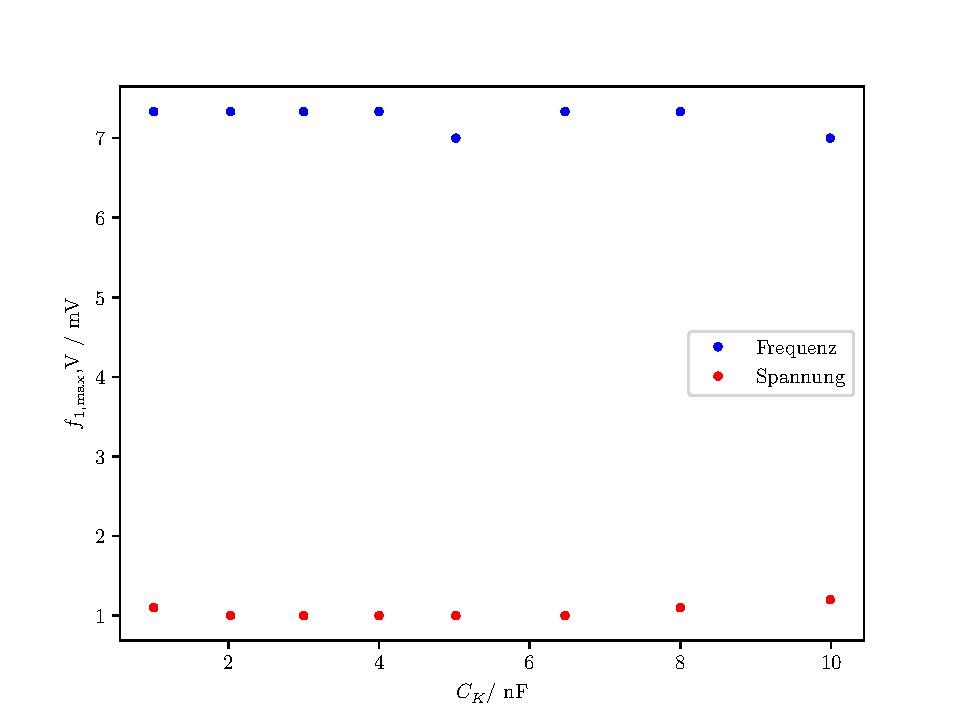
\includegraphics{freq1.pdf}
  \caption{Die aufgenommenen Messwerte zu c).}
  \label{fig:freq1}
\end{figure}

\begin{figure}[H]
  \centering
  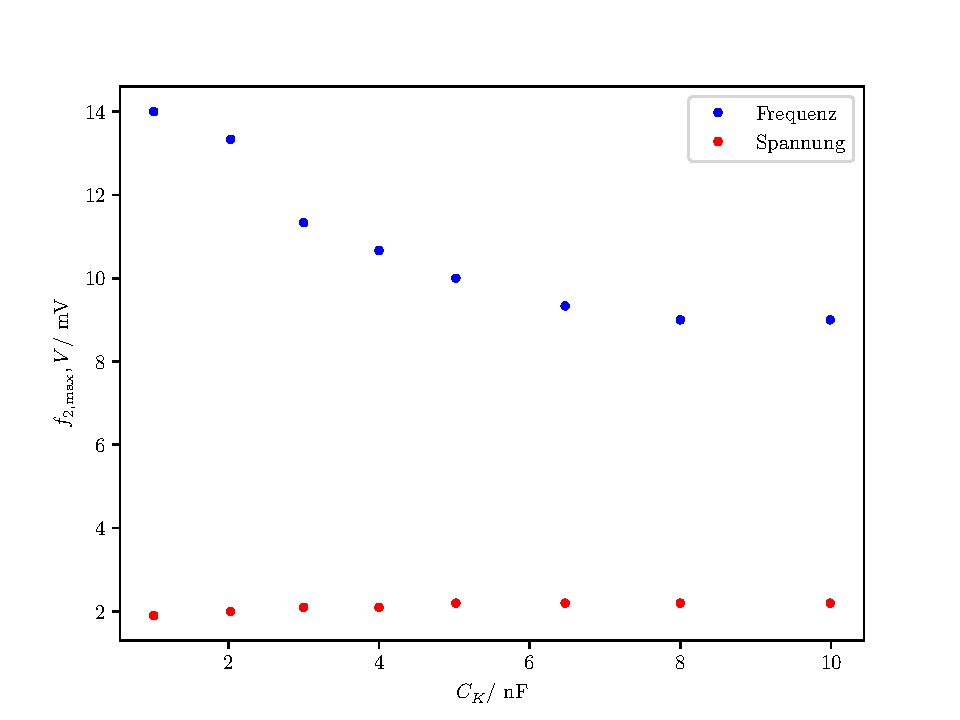
\includegraphics{freq2.pdf}
  \caption{Die aufgenommenen Messwerte zu c).}
  \label{fig:freq2}
\end{figure}

\noindent Die theoretischen Werte des Stromes $I_{2,\text{theo}}$ werden mithilfe des Widerstandes $R= 48 \,\upOmega$ durch die Formel $U=RI$ berechnet. 
Die Frequenzen der beiden Fundamentalschwingungen berechnen sich durch \autoref{eqn:funda1} und \autoref{eqn:funda2}, wobei die geringen Kapazitäten 
der beiden Spulen ebenfalls berücksichtigt wurden.
\begin{equation}
  \label{eqn:funda1}
  f_+ = \frac{1}{2\pi\sqrt{L(C + C_\text{Sp})}}
\end{equation} 
und \newline
\begin{equation}
  \label{eqn:funda2}
  f_- = \frac{1}{2\pi\sqrt{L\Bigl(\dfrac{CC_\text{K}}{2C+C_\text{K}} + C_\text{Sp}\Bigr)}}.
\end{equation}


\begin{table}[H]
  \centering
  \caption{Die erwarteten Theoriewerte.}
  \label{tab:theorietabelle}
  \begin{tabular}{c c c c c c c}
      \toprule
      $C_{\text{K}} \:/\: \si{\nano\farad}$ & $f_+ \:/\: \si{\kilo\hertz}$ & $f_{+, \text{theo}} \:/\: \si{\kilo\hertz}$ & $f_- \:/\: \si{\kilo\hertz}$ & $f_{-, \text{theo}} \:/\: \si{\kilo\hertz}$ & $I_2 \:/\: \si{\milli\ampere}$ & $I_{2,\text{theo}} \:/\: \si{\milli\ampere}$ \\
      \midrule
      9.99 & 38 & 35.32 & 49 & 32.80 & 1.1445 & 2.292 \\
      8.00 & 40 & 35.32 & 50 & 33.33 & 1.1449 & 2.292 \\
      6.47 & 40 & 35.32 & 50 & 33.95 & 1.1452 & 2.292 \\
      5.02 & 38 & 35.32 & 55 & 34.85 & 1.1455 & 2.292 \\
      4.00 & 40 & 35.32 & 58 & 35.85 & 1.0935 & 2.188 \\
      3.00 & 40 & 35.32 & 62 & 37.41 & 1.0936 & 2.188 \\
      2.03 & 40 & 35.32 & 73 & 40.19 & 1.0416 & 2.083 \\
      1.01 & 40 & 35.32 & 76 & 47.52 & 0.9896 & 1.979 \\
      \bottomrule
  \end{tabular}
\end{table}

\pagebreak